\section{Resultados}

Este estudio explora las interacciones génicas asociadas al Signo de Hoffmann con el fin de identificar patrones relevantes que contribuyan a la comprensión de su rol en enfermedades neurodegenerativas. Se aplicaron técnicas de propagación de red para añadir genes adicionales y se realizaron análisis topológicos y de enriquecimiento funcional para determinar las funciones biológicas y vías metabólicas implicadas.

\subsection{Red de interacción entre genes}


Se obtienen 46 genes relacionados con el termino del signo de Hoffmann de HPO, a los cuales se le aplica propagación de red mediante DIAMOnD hasta establecer 66 genes (20 genes añadidos).


\subsection{Propiedades de la red y detección de comunidades}

En el análisis de la red generada a partir de los genes asociados al signo de Hoffmann, se identificaron las siguientes propiedades generales de la red (ver Tabla \ref{tab:propiedades_red}):

\begin{table}[h!]
	\centering
	\caption{Propiedades generales de la red}
	\label{tab:propiedades_red}
	\begin{tabular}{|l|c|}
		\hline
		\textbf{Propiedad} & \textbf{Valor} \\ \hline
		\hline
		Número de nodos & 63 \\ \hline
		Número de aristas & 439 \\ \hline
		Grado promedio & 13.94 \\ \hline
		Densidad de la red & 0.22 \\ \hline
		Modularidad & 0.41 \\ \hline
	\end{tabular}
\end{table}


La modularidad de la red, calculada como 0.41, indica una estructura modular moderada con comunidades bien definidas. En total, se detectaron siete comunidades principales, cuyos tamaños se presentan en la Tabla \ref{tab:modularidad_comunidades}.

\begin{table}[h!]
	\centering
	\caption{Tamaños de las comunidades detectadas en la red}
	\label{tab:modularidad_comunidades}
	\begin{tabular}{|c|c|}
		\hline
		\textbf{Comunidad} & \textbf{Tamaño} \\ 
		& \textbf{(Número de nodos)} \\ \hline
		1 & 20 \\ \hline
		2 & 3 \\ \hline
		3 & 32 \\ \hline
		4 & 2 \\ \hline
		5 & 2 \\ \hline
		6 & 2 \\ \hline
		7 & 2 \\ \hline
	\end{tabular}
\end{table}



Para evaluar el papel estructural de los genes en la red, se calcularon métricas topológicas como la centralidad de cercanía y la centralidad de intermediación. Los resultados para los cinco nodos principales en cada métrica se presentan en las Tablas \ref{tab:centralidad_cercania} y \ref{tab:centralidad_intermediacion}.

\begin{table}[h!]
	\centering
	\begin{minipage}{0.48\textwidth}
		\centering
		\caption{Top 5 nodos con mayor centralidad de cercanía}
		\label{tab:centralidad_cercania}
		\begin{tabular}{|l|c|}
			\hline
			\textbf{Gen} & \textbf{Centralidad de cercanía} \\ 
			\hline
			DAO          & 1.0000                           \\ \hline
			COQ4         & 1.0000                           \\ \hline
			ERBB4        & 1.0000                           \\ \hline
			COQ7         & 1.0000                           \\ \hline
			OPTN         & 0.0108                           \\ \hline
		\end{tabular}
	\end{minipage}
	\hfill
	\begin{minipage}{0.48\textwidth}
		\centering
		\caption{Top 5 nodos con mayor centralidad de intermediación}
		\label{tab:centralidad_intermediacion}
		\begin{tabular}{|l|c|}
			\hline
			\textbf{Gen} & \textbf{\begin{tabular}[c]{@{}c@{}}Centralidad de\\ intermediación\end{tabular}} \\ 
			\hline
			RAB11A       & 208.26                                 \\ \hline
			UNC13A       & 188.01                                 \\ \hline
			VCP          & 148.44                                 \\ \hline
			DCTN1        & 139.38                                 \\ \hline
			PON1         & 112.00                                 \\ \hline
		\end{tabular}
	\end{minipage}
\end{table}


\subsubsection{Clustering}

El análisis se centró en los clusters 1 (rojo) y 3 (verde) debido a su relevancia en la red \ref{fig:Clustering}. El cluster 1 fue identificado como el más denso y cohesivo, lo que sugirió que agrupaba nodos funcionalmente importantes o vinculados a un proceso biológico clave. Por su parte, el cluster 3, aunque similar en tamaño, estuvo estrechamente relacionado espacialmente con el cluster 1, indicando una posible conexión funcional entre ambos. Los clusters restantes resultaron ser más pequeños, dispersos o menos relevantes, lo que justificó no priorizarlos en el análisis.

\begin{figure}[h!]
	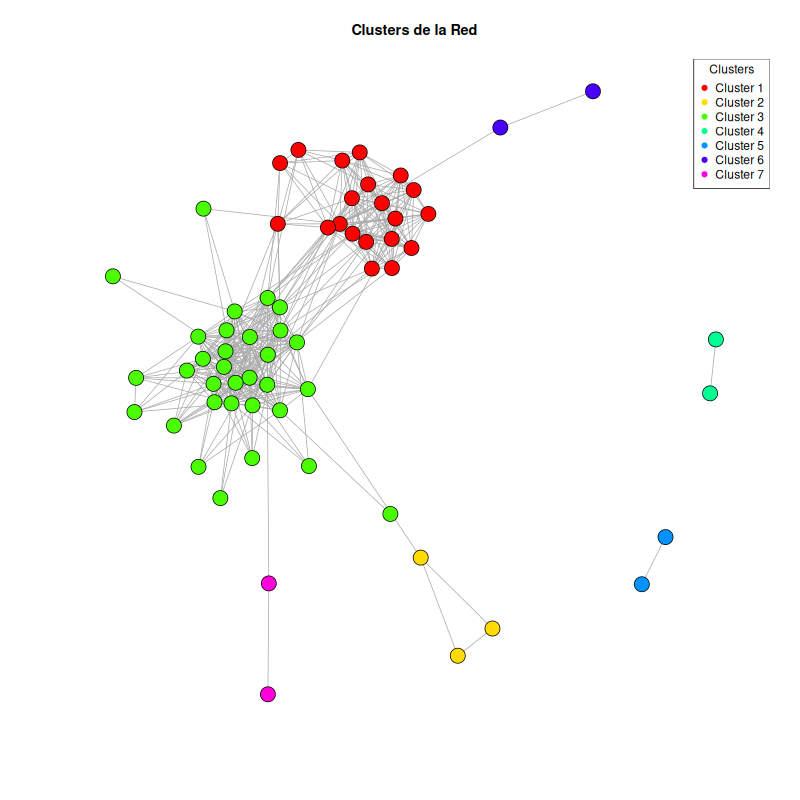
\includegraphics[width=0.8\textwidth]{figures/network_clusters_colored.png}
	\caption{Clustering por Louvain}
	\label{fig:Clustering}
\end{figure}



\subsection{Análisis de enriquecimiento funcional}

Se obtenieron resultados significativos para los clusters uno y tres, que son los que más número de genes albergan. En las figuras \ref{tb:c1_t1}, \ref{tb:c1_t2}, \ref{tb:c1_t3}, \ref{tb:c1_t4}, \ref{tb:c2_t1}, \ref{tb:c2_t2}, \ref{tb:c2_t3}, \ref{tb:c2_t4} se muestran los resultados más significativos por cada clúster y categoría.
\begin{table}[H]
	\centering
	\caption{Análisis de Enriquecimiento - GO Biological Process - Cluster 1}
	\label{tb:c1_t1}
	\begin{tabular}{|p{4cm}|p{4cm}|p{3cm}|}
		\hline
		\textbf{Término} & \textbf{Genes} & \textbf{p-value} \\ \hline
		Golgi to plasma membrane transport (GO:0006893) & RAB10, EXOC8, EXOC6B, EXOC4, EXOC6, EXOC5, EXOC2, EXOC1 & 7.33e-17 \\ \hline
		cilium organization (GO:0044782) & ARF4, EXOC8, EXOC7, RAB3IP, ASAP1, RAB11A, EXOC4, EXOC3, EXOC6, EXOC5, RAB11FIP3, RAB8A, EXOC2, EXOC1 & 1.53e-23 \\ \hline
		plasma membrane bounded cell projection assembly (GO:0120031) & ARF4, EXOC8, EXOC7, RAB3IP, ASAP1, RAB11A, EXOC4, EXOC3, EXOC6, EXOC5, RAB11FIP3, RAB8A, EXOC2, EXOC1 & 2.60e-22 \\ \hline
	\end{tabular}
\end{table}

\begin{table}[H]
	\centering
	\caption{Análisis de Enriquecimiento - GO Cellular Component - Cluster 1}
	\label{tb:c1_t2}
	\begin{tabular}{|p{4cm}|p{4cm}|p{3cm}|}
		\hline
		\textbf{Término} & \textbf{Genes} & \textbf{p-value} \\ \hline
		insulin-responsive compartment (GO:0032593) & RAB10, MYO5A & 3.41e-05 \\ \hline
		recycling endosome (GO:0055037) & RAB10, MYO5A, RAB11FIP3, RAB11A, RAB8A & 2.65e-07 \\ \hline
		recycling endosome membrane (GO:0055038) & RAB11FIP3, RAB11A, RAB8A & 2.55e-05 \\ \hline
	\end{tabular}
\end{table}

\begin{table}[H]
	\centering
	\caption{Análisis de Enriquecimiento - GO Molecular Function - Cluster 1}
	\label{tb:c1_t3}
	\begin{tabular}{|p{4cm}|p{4cm}|p{3cm}|}
		\hline
		\textbf{Término} & \textbf{Genes} & \textbf{p-value} \\ \hline
		myosin V binding (GO:0031489) & RAB10, RAB11A, RAB8A & 3.86e-07 \\ \hline
		myosin binding (GO:0017022) & RAB10, RALA, RAB11A, RAB8A & 2.58e-07 \\ \hline
		small GTPase binding (GO:0031267) & EXOC8, EXOC4, MYO5A, EXOC5, RAB11FIP3, RAB8A, EXOC2 & 2.45e-10 \\ \hline
	\end{tabular}
\end{table}

\begin{table}[H]
	\centering
	\caption{Análisis de Enriquecimiento - KEGG Pathways - Cluster 1}
	\label{tb:c1_t4}
	\begin{tabular}{|p{4cm}|p{4cm}|p{3cm}|}
		\hline
		\textbf{Término} & \textbf{Genes} & \textbf{p-value} \\ \hline
		Endocytosis & RAB10, ASAP1, RAB11FIP3, ARF5, RAB11A, RAB8A & 1.04e-07 \\ \hline
		Pancreatic cancer & RALA, IKBKG & 0.00252 \\ \hline
		Pancreatic secretion & RAB11A, RAB8A & 0.00426 \\ \hline
	\end{tabular}
\end{table}


\begin{table}[H]
	\centering
	\caption{Análisis de Enriquecimiento - Procesos Biológicos (GO:BP) - Cluster 3}
	\label{tb:c2_t1}
	\begin{tabular}{|p{4cm}|p{4cm}|p{3cm}|}
		\hline
		\textbf{Término} & \textbf{Genes} & \textbf{p-value} \\ \hline
		Positive regulation of ATP biosynthetic process (GO:2001171) & VCP, TREM2, PPARGC1A & 3.10e-07 \\ \hline
		Positive regulation of purine nucleotide biosynthetic process (GO:1900373) & VCP, TREM2, PPARGC1A & 1.05e-06 \\ \hline
		Regulation of ATP biosynthetic process (GO:2001169) & VCP, TREM2, PPARGC1A & 2.05e-06 \\ \hline
	\end{tabular}
\end{table}

\begin{table}[H]
	\centering
	\caption{Análisis de Enriquecimiento - Componentes Celulares (GO:CC) - Cluster 3}
	\label{tb:c2_t2}
	\begin{tabular}{|p{4cm}|p{4cm}|p{3cm}|}
		\hline
		\textbf{Término} & \textbf{Genes} & \textbf{p-value} \\ \hline
		Intracellular non-membrane-bounded organelle (GO:0043232) & FIG4, GLE1, VCP, TAF15, DCTN1, ANXA11, ANG, NEFH & 3.72e-04 \\ \hline
		Mitochondrial intermembrane space (GO:0005758) & CHCHD10, SOD1 & 3.88e-03 \\ \hline
		Organelle envelope lumen (GO:0031970) & CHCHD10, SOD1 & 4.70e-03 \\ \hline
	\end{tabular}
\end{table}


\begin{table}[H]
	\centering
	\caption{Análisis de Enriquecimiento - Funciones Moleculares (GO:MF) - Cluster 3}
	\label{tb:c2_t3}
	\begin{tabular}{|p{4cm}|p{4cm}|p{3cm}|}
		\hline
		\textbf{Término} & \textbf{Genes} & \textbf{p-value} \\ \hline
		Polyubiquitin modification-dependent protein binding (GO:0031593) & VCP, SQSTM1, OPTN, UBQLN2 & 1.28e-06 \\ \hline
		miRNA binding (GO:0035198) & MATR3, HNRNPA1 & 1.05e-03 \\ \hline
		Regulatory RNA binding (GO:0061980) & MATR3, HNRNPA1 & 1.86e-03 \\ \hline
	\end{tabular}
\end{table}

\begin{table}[H]
	\centering
	\caption{Análisis de Enriquecimiento - Rutas KEGG - Cluster 3}
	\label{tb:c2_t4}
	\begin{tabular}{|p{4cm}|p{4cm}|p{3cm}|}
		\hline
		\textbf{Término} & \textbf{Genes} & \textbf{p-value} \\ \hline
		Amyotrophic lateral sclerosis (ALS) & NEFH, SOD1, PRPH & 7.35e-05 \\ \hline
		Mitophagy & TBK1, SQSTM1, OPTN & 1.52e-04 \\ \hline
		Huntington disease & DCTN1, PPARGC1A, SOD1 & 3.57e-03 \\ \hline
	\end{tabular}
\end{table}






